\chapter{Implementasi dan Pengujian}
\label{chap:implementasi_pengujian}

\section{Implementasi}

Implementasi dilakukan di dua buah mesin. Implementasi pertama dilakukan pada komputer peneliti untuk keperluan pengujian fungsional. Komputer tersebut memiliki spesifikasi seperti berikut:

\begin{itemize}
	\item Prosesor: 1.80 GHz
	\item RAM: 4.00 GB
	\item Sistem Operasi: Windows 8.1 Pro (64-bit)
\end{itemize}

Implementasi berikutnya dilakukan pada sebuah mesin virtual yang dibuat pada \textit{platform Windows Azure}. Mesin virtual ini terhubung ke internet serta beroperasi 24 jam sehingga dapat melayani permintaan tanpa henti. Adapun spesifikasi dari mesin virtual ini adalah sebagai berikut:

\begin{itemize}
	\item Prosesor: 1 core
	\item RAM: 1.75 GB
	\item Hard disk: 28.8 GB
	\item Sistem Operasi: Ubuntu 14.04.2 LTS (64-bit)
\end{itemize}

\section{Pengujian}

\subsection{Pengujian Fungsional}

TODO

\subsection{Pengujian Eksperimental}

Pengujian eksperimental dibagi menjadi 3 tahap:

\begin{enumerate}
	\item Survei \textit{online} terhadap kepuasan kualitas pencarian pengguna, dan potensi keinginan untuk berkontribusi selama satu bulan.
	\item Kampanye fitur integrasi perbaikan rute melalui Facebook selama satu bulan.
	\item Survei \textit{online} terhadap kepuasan kualitas pencarian serta keterlibatan pengguna dalam perbaikan rute.
\end{enumerate}

Ketiga tahap tersebut dijelaskan pada subbab-subbab berikut.

\subsubsection{Tahap 1: Survei Kepuasan Kualitas Pencarian dan Potensi Keinginan Berkontribusi}

Pada tahap ini, peneliti membuat survei \textit{online} memanfaatkan aplikasi Google Docs\footnote{\url{https://google.com/docs}}. Ada 6 pertanyaan yang ditanyakan, yaitu:

\begin{itemize}
	\item \textbf{Seberapa baik rute kami secara keseluruhan?} (mengerikan / buruk / netral / baik / sempurna)
	\item \textbf{Seberapa baik rute kami pada bagian rute kendaraan?} (mengerikan / buruk / netral / baik / sempurna)
	\item \textbf{Seberapa baik rute kami pada bagian rute berjalan?} (mengerikan / buruk / netral / baik / sempurna)
	\item \textbf{Di kota apa Anda menggunakan KIRI?} (Bandung / Jakarta / Malang / Surabaya)
	\item \textbf{Di mana Anda tinggal?} (Bandung / Jakarta / Malang / Surabaya)
	\item \textbf{Apakah Anda tertarik untuk berkontribusi data rute?} (Ya, dengan imbalan / Ya, tanpa syarat / Tidak / Tidak tahu)
\end{itemize}

Survei ini disediakan \textit{online} pada alamat \url{http://goo.gl/forms/WkeU8oK4Ek}, dan ditunjukkan pada situs web KIRI setelah hasil pencarian ditampilkan (Gambar \ref{fig:5_survei_1}) selama bulan April 2015.

\begin{figure}
	\centering
	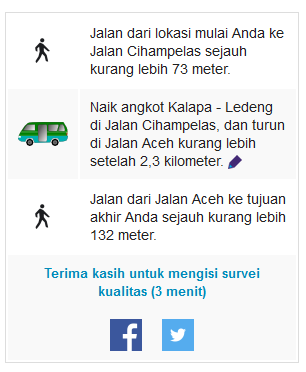
\includegraphics[scale=0.75]{Gambar/5_survei_1}
	\caption{Tautan ke Survei Tahap 1} 
	\label{fig:5_survei_1}
\end{figure}

Setelah masa survei berakhir, didapatkan 33 responden survei. Dari segi kualitas pencarian (Gambar \ref{fig:5_hasilsurvei_1_1}), secara umum pengguna puas dengan hasil kualitas pencarian, ditandai dengan sebagian besar pengguna memilih "baik" pada ketiga jenis pertanyaan. Pada bagian kualitas rute kendaraan, relatif lebih banyak pengguna yang memilih "sempurna" dibandingkan dengan rute berjalan. Peneliti menduga bahwa ini dikarenakan oleh dua hal:

\begin{itemize}
	\item Pencarian rute di KIRI relatif lebih baik dibandingkan dengan pada situs web sejenis\footnote{\url{http://angkot.tibandung.com/}}, karena lebih presisi hingga titik koordinat.
	\item Karena keterbatasan data, hasil rute berjalan di KIRI menghasilkan garis lurus dan tidak mengikuti arah jalan yang sesungguhnya.
\end{itemize}

Dari segi demografi pengguna (Gambar \ref{fig:5_hasilsurvei_1_2}, sebagian besar pengguna menggunakan KIRI di Bandung dan tinggal di Bandung. Hal ini memberikan dua keuntungan kepada peneliti:

\begin{itemize}
	\item Sesuai dengan batasan masalah, yaitu penelitian dilakukan di kota Bandung.
	\item Pengguna relatif mengenal rute transportasi publik di Bandung, karena tinggal di kota Bandung.
\end{itemize}

Terakhir, survei mengenai potensi keinginan berkontribusi (Gambar \ref{fig:5_hasilsurvei_1_3}) memberikan hasil yang bervariasi. Sebagian besar responden bersedia memperbaiki rute yang salah, namun ada juga yang berharap imbalan maupun tidak berminat. Hasil tersebut cukup meyakinkan peneliti bahwa pada tahap berikutnya akan ada sebagian dari pengguna yang bersedia memperbaiki.

\begin{figure}
	\centering
	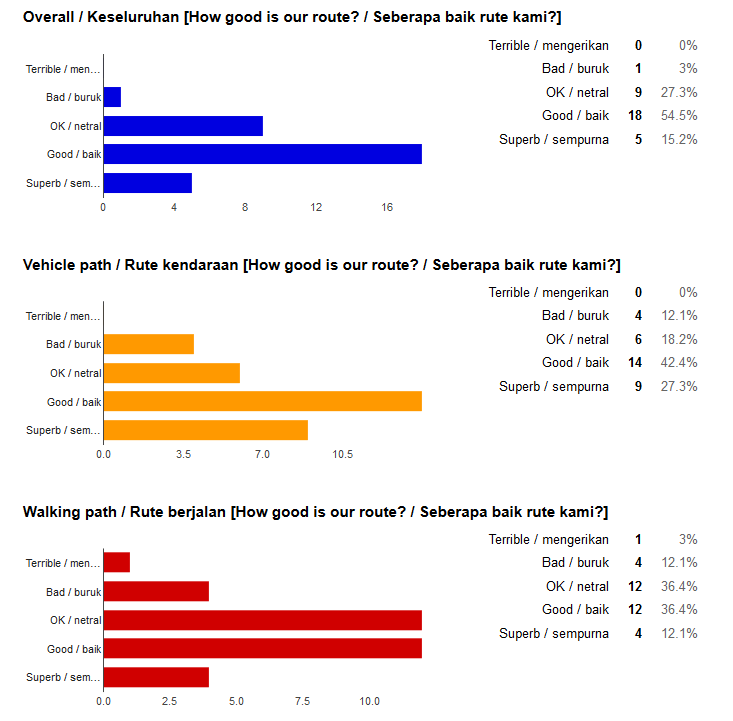
\includegraphics[scale=0.75]{Gambar/5_hasilsurvei_1_1}
	\caption{Hasil Survei Tahap 1 (Kualitas Pencarian)} 
	\label{fig:5_hasilsurvei_1_1}
\end{figure}

\begin{figure}
	\centering
	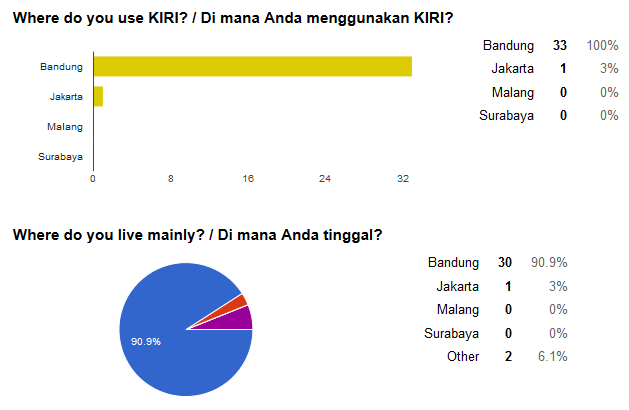
\includegraphics[scale=0.75]{Gambar/5_hasilsurvei_1_2}
	\caption{Hasil Survei Tahap 1 (Demografi Pengguna)} 
	\label{fig:5_hasilsurvei_1_2}
\end{figure}

\begin{figure}
	\centering
	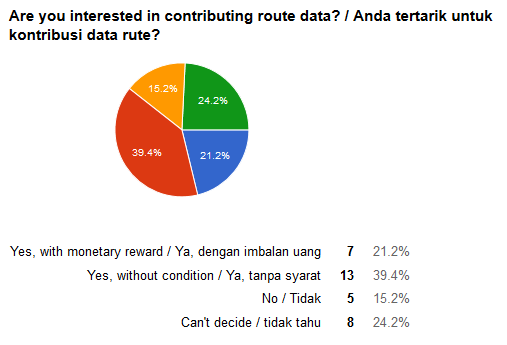
\includegraphics[scale=0.75]{Gambar/5_hasilsurvei_1_3}
	\caption{Hasil Survei Tahap 1 (Kesediaan Berkontribusi)} 
	\label{fig:5_hasilsurvei_1_3}
\end{figure}